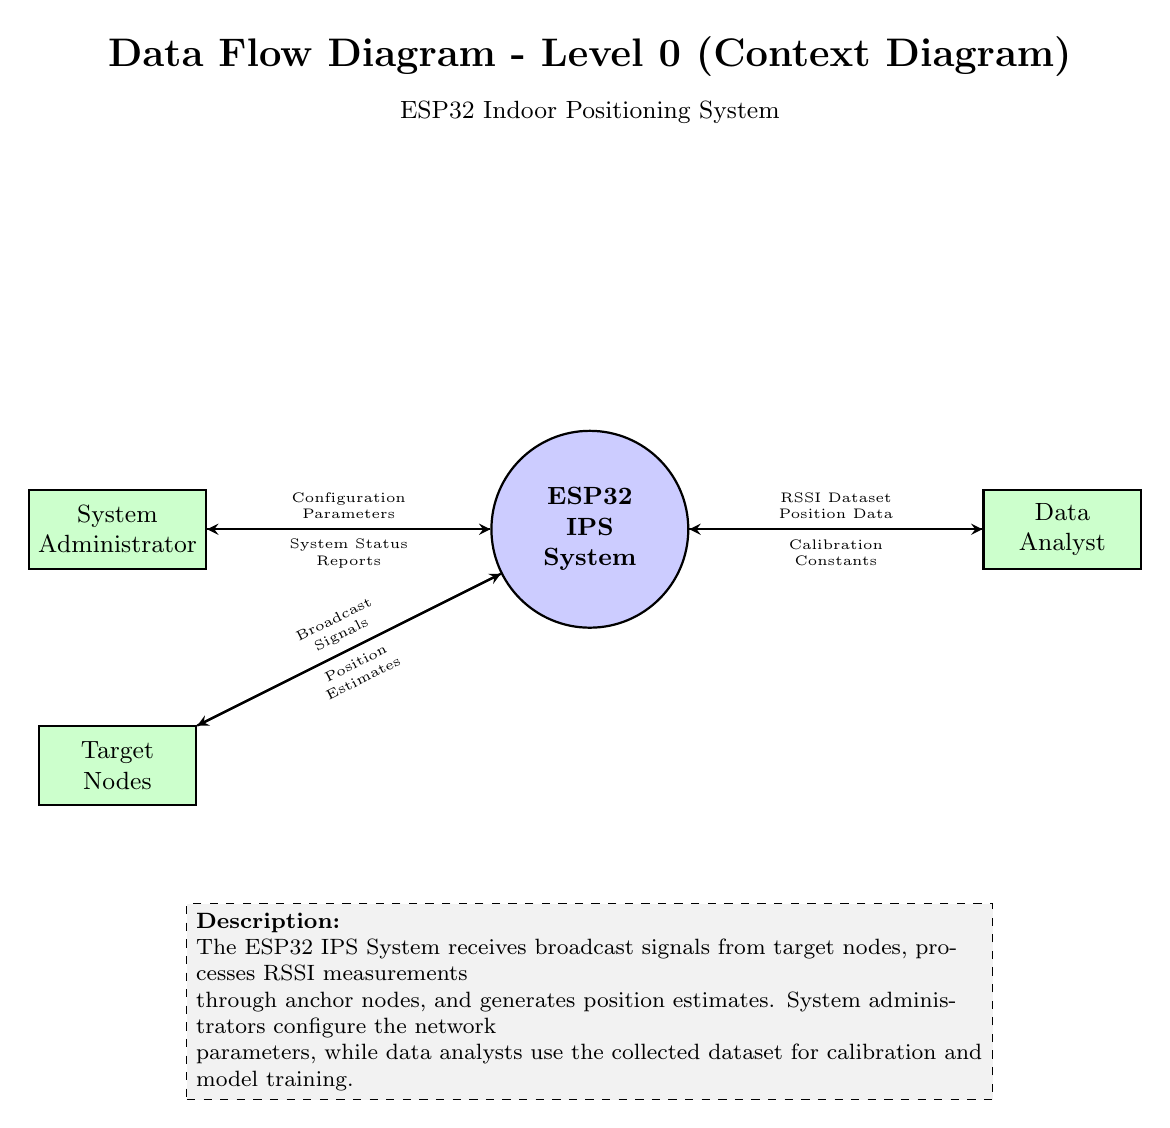
\begin{tikzpicture}[
    node distance=3cm,
    process/.style={circle, draw, thick, minimum size=2.5cm, align=center, font=\small\bfseries, fill=blue!20},
    entity/.style={rectangle, draw, thick, minimum width=2cm, minimum height=1cm, align=center, font=\small, fill=green!20},
    datastore/.style={rectangle, draw, thick, minimum width=2.5cm, minimum height=0.8cm, align=center, font=\small, fill=yellow!20},
    flow/.style={->, thick, >=stealth}
]

% Title
\node[font=\Large\bfseries] at (0,6) {Data Flow Diagram - Level 0 (Context Diagram)};
\node[font=\small] at (0,5.3) {ESP32 Indoor Positioning System};

% External Entities
\node[entity] (user) at (-6,0) {System\\Administrator};
\node[entity] (target) at (-6,-3) {Target\\Nodes};
\node[entity] (analyst) at (6,0) {Data\\Analyst};

% Central Process
\node[process] (system) at (0,0) {ESP32\\IPS\\System};

% Data Flows
\draw[flow] (user) -- node[above, font=\tiny, sloped, align=center] {Configuration\\Parameters} (system);
\draw[flow] (system) -- node[below, font=\tiny, sloped, align=center] {System Status\\Reports} (user);

\draw[flow] (target) -- node[above, font=\tiny, sloped, align=center] {Broadcast\\Signals} (system);
\draw[flow] (system) -- node[below, font=\tiny, sloped, align=center] {Position\\Estimates} (target);

\draw[flow] (system) -- node[above, font=\tiny, sloped, align=center] {RSSI Dataset\\Position Data} (analyst);
\draw[flow] (analyst) -- node[below, font=\tiny, sloped, align=center] {Calibration\\Constants} (system);

% Description box
\node[rectangle, draw, dashed, fill=gray!10, text width=10cm, align=left, font=\footnotesize] at (0,-6) {
    \textbf{Description:}\\
    The ESP32 IPS System receives broadcast signals from target nodes, processes RSSI measurements\\
    through anchor nodes, and generates position estimates. System administrators configure the network\\
    parameters, while data analysts use the collected dataset for calibration and model training.
};

\end{tikzpicture}
